%-----------------begin---preamble-------------------
\documentclass{article}
\usepackage{amsmath,amssymb,amsthm}
\usepackage{tikz,tkz-euclide}
\usepackage{marginnote}
\usepackage{float}
\usepackage[margin=0.8in]{geometry}
% \usepackage{enumerate}


\usetikzlibrary{calc,patterns,angles,quotes}
\usetkzobj{all}

\def\deg{^{\circ}}
\newcommand\heading[1]{\ \\\large{\textbf{#1}}}
\newcommand\ora[1]{\overrightarrow{#1}}

\newtheorem*{problem}{Problem}
%------------------end---preamble--------------------

\begin{document}
	\begin{problem}[Hong Kong TST 2,2017]
		\ \\\\
		Let $ABC$ be a triangle with AB=AC. A circle $\Gamma$ lies outside triangle $ABC$ and is tangent to line $AC$ at $C$. Point $D$ lies on $\Gamma$ such that the circumcircle of $ABD$ is internally tangent to $\Gamma$. Segment $AD$ meets $\Gamma$ again at $E$. Prove that $BE$ is tangent to $\Gamma$.
	\end{problem}
	\begin{proof}
		
	\begin{figure}[H]
	\begin{center}
	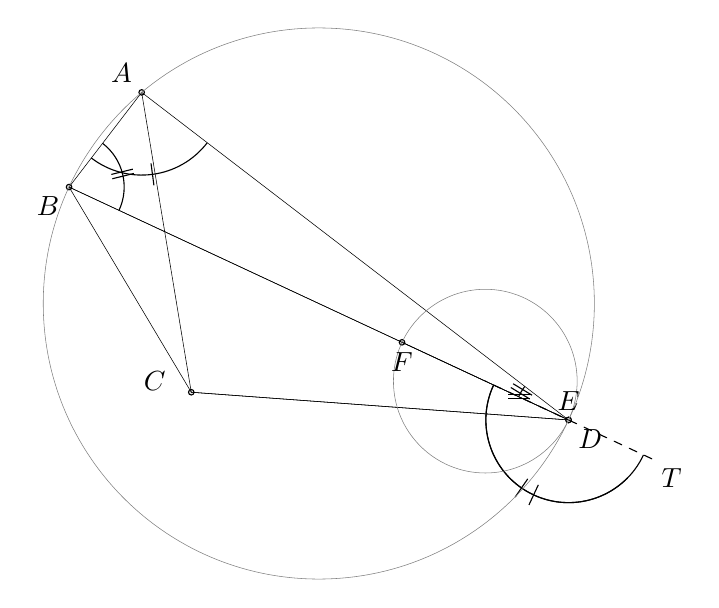
\begin{tikzpicture}[scale=3.5]
		% \useasboundingbox (-2,-2) rectangle  (2,2);
		\tkzDefPoint(0,0){O}
		\tkzDefPoint[label=120:$A$](130:1){A}
		\tkzDefPoint[label=-60:$D$](-25:1){D}
		\tkzDefBarycentricPoint(D=2,O=1) \tkzGetPoint{I}
		\tkzInterLC(D,A)(I,D)\tkzGetFirstPoint{E}
		\tkzTangent[at=E](I)\tkzGetPoint{t}
		\tkzInterLC(E,t)(O,A)\tkzGetSecondPoint{B}
		\tkzInterCC(A,B)(I,D)\tkzGetSecondPoint{C}
		\tkzInterLC(D,B)(I,D)\tkzGetSecondPoint{F}
		\tkzTangent[at=D](O)\tkzGetPoint{s}
		\tkzDefPointsBy[symmetry=center D](s){s1}
		\tkzMarkAngles[size=0.3,mark=|](B,A,D F,E,D B,D,s1)
		\tkzMarkAngles[size=0.2,mark=||](E,B,A B,E,F A,D,F)
		\tkzLabelPoint[below right](s1){$T$}
		\tkzDrawPoints(A,B,C,D,E,F)
		\tkzDrawSegments(A,B A,C A,E B,C B,E B,F C,D C,E D,E D,F E,F)
		\tkzDrawCircle(O,A)
		\tkzDrawCircle(I,D)
		\tkzLabelPoints[above](E)
		\tkzLabelPoints[below left](B)
		\tkzLabelPoints[below](F)
		\tkzLabelPoints[above left=-0.1 and 0.2](C)
		\tkzDrawLine[thin,dashed,add=1 and 0](D,s)
		\end{tikzpicture}
	\end{center}		
	\end{figure}
	First construct point $F$ as the intersection of $\Gamma$ and $BD$. Let $T$ be a point on the tangent of $\Gamma$ at $D$, such that $\angle BDT$ is acute.\\

	Using the fact that $TD$ is tangent to $\Gamma$ and the circumcircle of $ABD$.
	\begin{flalign}
		\angle FED=\angle BDT=\angle BAD \nonumber
	\end{flalign}

	So $AB||EF$.\marginnote{(1)}\\

	Using power of a point,the fact that $AC$ is tangent to $\Gamma$, and that $AC=AB$.
	\begin{flalign}
		AB^2=AC^2=DA \cdot AE \nonumber
	\end{flalign}

	So $AB$ is tangent to the circumcircle of $EBD$.\marginnote{(2)}\\

	Now, combining (1) and (2):
	\begin{flalign}
		\angle BEF=\angle EBA=\angle EDB=\angle EDF\nonumber
	\end{flalign}
	
	Thus, since $\angle BEF=\angle EDB \nonumber$, we have $BE$ is tangent to $\Gamma$, by the converse of Tan-Chord Th\textsuperscript{\underline{m}}.
	\end{proof}
	
	
\end{document}